Une enceinte calorifugée (qui évite les transferts thermiques) à parois rigides est partagée en deux par une paroi amovible. Cette paroi est enlevable sans apporter de travail mécanique.

\begin{center}
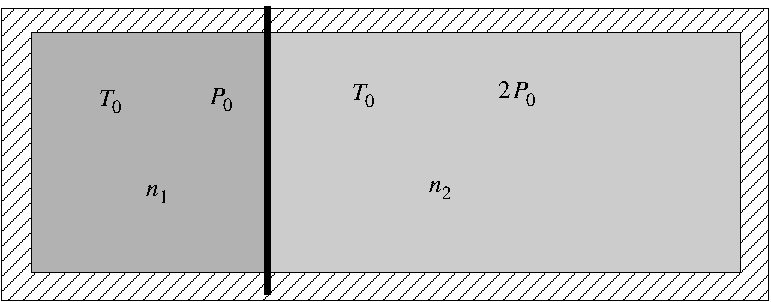
\includegraphics[scale=0.8]{../Fig/DetenteIsoleeSurReseau}
\end{center}

Initialement, à l'état~A, la paroi est en place, il y a donc deux
compartiments.
Ils sont
remplis du même gaz monoatomique que l'on assimile à un gaz parfait (sans interactions). La température est la même des deux
côtés: $T_0$. À gauche, il y a $n_1$ moles dans un volume $V_1$; à
droite, $n_2$ moles dans un volume $V_2$. Enfin, la pression est double
à droite par rapport à gauche. $P_1 = P_0$, $P_2 = 2 P_0$.

On enlève alors la paroi, les deux gaz se mélangent pour arriver à l'état d'équilibre B.\\
On cherche à déterminer l'état final et la variation d'entropie de la
transformation de deux manières différentes : tout d'abord par un
raisonnement de thermodynamique macroscopique, ensuite par une
modélisation microscopique.

\medskip

\tiret{Approche thermodynamique macroscopique}


\question
On pose $x$ tel que $n_2 = x n_1$.
Calculer les volumes initiaux~$V_1$ et~$V_2$ en fonction de $x$,
$n_1$, $T_0$, $P_0$.
\reponse{
Il faut reprendre les résultats de la question~1:
$$ V_1 =  {n_1 R T_0 \over P_0} \qquad \text{et} \qquad V_2 = {xn_1 R T_0 \over 2 P_0} = {x \over 2}  V_1 $$
}


\question
Utiliser le premier principe de la thermodynamique pour déterminer l'état final du gaz: pression et température finales~$P_B$ et $T_B$ en fonction de $T_0$, $P_0$ et $x$. On rappelle que l'énergie interne molaire d'un gaz parfait ne dépend que de sa température.
\reponse{
Il s'agit simplement d'une généralisation de la détente de Joule-Gay-Lussac. Elle est adiabatique et sans travail fourni, donc à énergie interne constante. L'énergie interne ne dépendant que de la température et celle-ci étant la même initialement de part et d'autre, alors elle reste constante: La température finale est donc $T_B =T_0$. Il est alors immédiat de calculer la pression finale puisque l'on connaît le nombre de moles: $n_1+n_2$ et le volume $V_1 + V_2$. Les volumes ne sont pas donnés dans l'énoncé mais il est immédiat de les calculer à partir des conditions initiales:
$$ V_1 =  {n_1 R T_0 \over P_0} \qquad \text{et} \qquad V_2 = {n_2 R T_0 \over 2 P_0} $$
Ainsi la pression finale $P_B$ est:
$$P_B = {(n_1 + n_2) R T_0 \over (V_1 + V_2)} = {(n_1 + n_2) R T_0 \over \displaystyle{{n_1 R T_0 \over P_0} + {n_2 R T_0 \over 2 P_0}} } = {n_1 + n_2 \over n_1 + n_2/2 } P_0$$
Il est facile de vérifier que $P_0 < P_B < 2 P_0$.
}
 

On admet l'expression suivante de l'entropie d'un gaz parfait monoatomique en fonction du nombre de mole $n$, de son volume $V$ et de sa température $T$: $$ S = nR \left[ \ln \left( {V\over n} \right) + {3\over 2} \ln ( T ) + K \right]  $$ où $K$ est une constante qui ne dépend que des constantes fondamentales et de la masse atomique du gaz


\reponse{
Dans les ouvrages on trouve souvent:
$$S = nR \left( \ln V + {3\over 2} \ln T \right) + cte(n) $$
où $cte$ est une fonction ne dépendant que de $n$ et des caractéristiques du gaz. Il est très maladroit de laisser $S$ sous cette forme car l'extensivité n'y apparaît pas. Il faut écrire une expression qui est extensive:
$$ S = nR \left[ \ln \left( {V\over n} \right) + {3\over 2} \ln T + K \right]  $$
Ici $K'$ est une vraie constante ne dépendant pas du nombre de moles mais seulement des constantes fondamentales et des caractéristiques du gaz\footnote{On montrera en cours de master qu'elle dépend uniquement de la masse atomique du gaz, de la constante de Boltzmann et de la constante de Planck.}.
}

\question
Écrire l'expression de l'entropie initiale $S_A$.
\reponse{
\begin{alignat*}{2}
S_A     &= &    &\  S_1 + S_2  \\
           & = &    & \  n_1 R\left[ \ln \left( {V_1\over n_1} \right) + {3\over 2} \ln T_0 + K  \right]\\
           &\  & +  &\   n_2 R\left[ \ln \left( {V_2\over n_2} \right) + {3\over 2} \ln T_0 + K  \right] 
\end{alignat*}
La constante $K$ est la même dans les deux termes car il s'agit du même gaz.
}

\question
Écrire l'expression de l'entropie finale $S_B$.
\reponse{
$$ S_B  =  (n_1  + n_2) R \left[ \ln \left( {V_1 + V_2 \over n_1 + n_2 } \right) + {3\over 2} \ln T_0 + K  \right] $$
}



\question
Calculer la variation d'entropie~$\Delta S$ en fonction de $n_1$ et de $x$. Montrer que $\Delta S= n_1 R\left[ (1+x )\ln  \left( {1 + {x/2} \over 1 + x } \right)  + x\ln 2 \right]$
\reponse{
On regroupe entre eux les deux termes en $n_1 R$ et les deux termes en $n_2 R$ en tenant compte de $n_2 = x n_1$ et $V_2 = x V_1 / 2$:
\begin{alignat*}{2}
\Delta S  &= &    &\  S_B - S_A  \\
              & = &    & \ n_1 R\left[ \ln \left( {V_1 + {x \over 2} V_1 \over n_1 + x n_1} \right) + {3\over 2} \ln T_0 + K  - \ln \left( {V_1\over n_1} \right) - {3\over 2} \ln T_0 - K \right]  \\
              &\  & +  &\   x n_1 R\left[ \ln  \left( {V_1 + {x \over 2} V_1 \over n_1+ x n_1} \right)+ {3\over 2} \ln T_0 + K  - \ln \left( {{x \over 2} V_1 \over x n_1} \right) - {3\over 2} \ln T_0 - K \right]  
\end{alignat*}
$V_1$ et $n_1$ disparaissent par soustraction de tous les logarithmes. Il reste seulement les termes en x:
\begin{align*}
 \Delta S & = n_1 R\left[ \ln  \left( {1 + {x/2} \over 1 + x } \right) \right]  + x n_1 R\left[ \ln  \left( {1 + {x/2} \over 1+ x} \right) - \ln \left( {{x/2} \over x } \right) \right] \\
               & = n_1 R\left[ (1+x )\ln  \left( {1 + {x/2} \over 1 + x } \right)  + x\ln 2 \right]
\end{align*}
}

%\question Faire trois applications numériques pour $x=0$, $x=1$ et $x=2$. Commenter à chaque fois le signe de~$\Delta S$ et éventuellement sa valeur.
%\reponse{ \noindent Pour $x=0$ on trouve $\Delta S=0$. C'est normal puisque $x=0$ signifie pas de compartiment~2 donc pas de transformation! \noindent Pour $x=1$ on trouve $\Delta S = 0{,}12 \times n_1 R > 0$. \noindent Pour $x=2$ on trouve $\Delta S = 0{,}17 \times n_1 R > 0$. On trouve à chaque fois $\Delta S > 0$: l'entropie augmente au cours de la transformation. C'est bien conforme au second principe puisque cette transformation est évidemment irréversible.
%}

\medskip

\tiret{Approche statistique microscopique}

On utilise ici une méthode dite de {\em gaz sur réseau}.
Chaque compartiment est découpé en un grand nombre de cellules, du 
même volume, en nombre
plus grand que le nombre de particules.
Ainsi, à gauche il y a initialement~$M_1$ cellules pour~$N_1$
particules, $M_1>N_1$; à droite~$M_2$ cellules pour~$N_2$ particules, $M_2>N_2$.
La règle de répartitions des particules est:~$0$ ou~$1$ particule par cellule. Comme la température et donc l'énergie ne jouent aucun rôle dans cette transformation, on s'intéresse uniquement à l'aspect configurations possibles des particules dans chaque compartiment.

\medskip

\question
On note~$\Omega_1$ et~$\Omega_2$ les nombres de micro-états initiaux distincts (distributions des particules dans chaque compartiment) à
gauche et à droite. Exprimer alors l'entropie initiale~$S_A$ en
fonction de~$\Omega_1$ et~$\Omega_2$.
\reponse{
$$ S_A = k \ln \Omega_1 + k \ln \Omega_2 $$
}

\question
Exprimer~$\Omega_1$ (respectivement~$\Omega_2$) sous forme de combinaisons en fonction de $M_1$ et $N_1$ (resp. $M_2$ et $N_2$)
\reponse{
$\Omega_1$ est le nombre de manière de choisir $N_1$ cellules parmi $M_1$ cellules. Cela s'écrit:
$$ \Omega_1 = \binom{M_1}{N_1} = {M_1 ! \over N_1 ! \, (M_1 - N_1) !} $$
De même:
$$ \Omega_2 = \binom{M_2}{N_2} = {M_2 ! \over N_2 ! \, (M_2 - N_2) !} $$
}

\question
Calculer alors $S_A$ en fonction des quatre nombres~$M_1$, $M_2$,
$N_1$ et~$N_2$.
\reponse{
Il faut développer les logarithmes des factorielles en utilisant la formule donnée dans l'énoncé.
\begin{alignat*}{2}
S_A/k     &= &    &\  S_1/k + S_2/k  \\
           & = &    & \  \ln M_1! - \ln N_1! - \ln(M_1-N_1)! \\
           &\  & +  &\   \ln M_2! - \ln N_2! - \ln(M_2-N_2)!  \\
           & = &  & \ M_1\ln M_1 - M_1 - N_1 \ln N_1 + N_1 - (M_1-N_1) \ln (M_1-N_1) + (M_1-N_1) \\
           &\ & + &\ M_2 \ln M_2 - M_2 - N_2 \ln N_2 + N_2 - (M_2-N_2) \ln (M_2-N_2) + (M_2-N_2) \\
           & = &  & \ M_1\ln M_1 - N_1 \ln N_1 - (M_1-N_1) \ln (M_1-N_1)  \\
           &\ & + &\ M_2 \ln M_2 - N_2 \ln N_2 - (M_2-N_2) \ln (M_2-N_2) 
\end{alignat*}
}

\question
Exprimer~$\Omega_B$, le nombre de micro-états du macro-état final.
\reponse{
Il s'agit ici de la répartition de $ N_1 + N_2$ particules dans $M_1 + M_2$ cases:
$$ \Omega_B = \binom{M_1 + M_2}{N_1 + N_2}  = {(M_1 + M_2)! \over (N_1+N_2)! \, (M_1 + M_2 - N_1 - N_2)!} $$
}

\question
Calculer alors $S_B$ en fonction des quatre nombres~$M_1$, $M_2$,
$N_1$ et~$N_2$.
\reponse{
À nouveau il faut développer les logarithmes des factorielles.
\begin{alignat*}{2}
S_B/k     &= &    & \  \ln (M_1+M_2) ! - \ln (N_1 + N_2)! - \ln(M_1 + M_2 - N_1 - N_2)! \\
           & = &  & \ (M_1+M_2)\ln (M_1+M_2) - M_1 - M_2 - (N_1+N_2) \ln (N_1 + N_2) + N_1 + N_2 \\ 
           & \ & - & \ (M_1 + M_2 - N_1 - N_2) \ln (M_1 + M_2 - N_1 - N_2) + M_1 + M_2 - N_1 - N_2 \\
           &= &  &\ (M_1+M_2)\ln (M_1+M_2) - (N_1+N_2) \ln (N_1 + N_2)  \\ 
           & \ & - & \ (M_1 + M_2 - N_1 - N_2) \ln (M_1 + M_2 - N_1 - N_2)   
\end{alignat*}
}

\question
On doit respecter la relation $\frac{M_2}{M_1}=\frac{V_2}{V_1}$. Déterminer la relation simple entre~$M_1$ et~$M_2$ en fonction de $x=\frac{N_2}{N_1}$, introduit en première partie.

\reponse{
À la partie précédente nous avons montré facilement, en utilisant l'équation d'état du gaz parfait que $\displaystyle V_2 = {x\over 2} V_1$. Puisque les cellules sont de même taille dans chaque compartiment, on a donc: $\displaystyle M_2 = {x\over 2} M_1$. 
}

\question
On introduit maintenant un coefficient de dilution $\alpha <1$ tel que
$N_1 = \alpha M_1$.
Écrire alors les trois nombres~$N_1$, $N_2$ et~$M_2$ uniquement en
fonction de~$M_1$, $x$ et~$\alpha$.
\reponse{
$\alpha$ indique la fraction de cellules occupées par une particule du gaz. Le cas très dilué correspond à $\alpha \ll 1$. $\alpha=1$ correspond à la situation de condensation maximale du modèle, lorsque les cellules sont toutes occupées en même temps.

$N_2$ est relié à $N_1$ par $x$: $N_2 = x N_1$. Comme $N_1 = \alpha M_1$, cela donne $N_1 = \alpha x M_1$. En résumé:
\begin{align*}
N_1  & = \alpha M_1  \\
N_2 & = \alpha x M_1 \\
M_2 & = {x\over 2} M_1
\end{align*}
$M_1$ peut alors se mettre en facteur de tous les termes, aussi bien à l'extérieur qu'à l'intérieur des logarithmes.
}

\question
Récrire avec ces notations les expressions de~$S_A$ et~$S_B$, puis la
variation d'entropie de la transformation. Ne pas développer les
logarithmes de produits, écrire simplement dans l'ordre les termes de la
différence $S_B - S_1 - S_2$ et vérifier alors que l'on obtient
directement:
\begin{align*}
{ \Delta S \over M_1 k_B} = &+ \left( 1 + {x\over 2} \right) \ln\left( 1
  + {x\over 2} \right) - \alpha (1+x) \ln [\alpha (1+x)] \\
  & -\left( 1 + {x\over 2} - \alpha(1+x) \right)
          \ln\left(1+ {x\over 2} - \alpha(1+x) \right) \\
          &+ \alpha \ln\alpha + (1-\alpha) \ln (1-\alpha) \\
          &- {x\over 2} \ln \left( {x\over 2} \right) + \alpha x \ln[\alpha x]
          + \left( {x\over 2} -\alpha x\right) \ln \left( {x\over 2}
          - \alpha x \right)
\end{align*}
\reponse{
En mettant $M_1$ en facteur partout, nous obtenons:
\begin{alignat*}{2}
S_A/k     &= &  & \ M_1\ln M_1 - \alpha M_1 \ln [\alpha M_1] - (M_1-\alpha M_1) \ln [M_1-\alpha M_1]  \\
           &\ & + &\ {x\over 2}M_1 \ln \left( {x\over 2} M_1 \right) - \alpha x M_1 \ln [\alpha x M_1 ] - \left({x\over 2 }M_1-\alpha x M_1 \right) \ln \left({x\over 2}M_1-\alpha x M_1 \right) 
\end{alignat*}
En développant les logarithmes, tous les termes en $\ln M_1$ s'annulent deux à deux. $M_1$ peut être mis en facteur, il reste:
\begin{alignat*}{2}
{S_A\over M_1 k }    &= &  & - \alpha \ln\alpha - (1-\alpha) \ln [1-\alpha]  \\
           &\ & + &\ {x\over 2}\ln \left( {x\over 2} \right) - \alpha x \ln [\alpha x] - \left({x\over 2 }-\alpha x \right) \ln \left({x\over 2}-\alpha x \right) 
\end{alignat*}
$S_B$ se calcule de la même manière, tous les termes en $\ln M_1$ s'annulant deux à deux.
\begin{alignat*}{2}
{S_B\over M_1 k}     &= &  &\ (1+x/2)\ln (1+x/2) - (\alpha+\alpha x) \ln (\alpha + \alpha x)  \\ 
           & \ & - & \ (1 + x/2 - \alpha - \alpha x) \ln (1 + x/2 - \alpha - \alpha x)   
\end{alignat*}
$\Delta S$ s'obtient en faisant la soustraction de ces deux dernières expressions:
\begin{alignat*}{2}
{\Delta S \over M_1 k}     &= &   &\  {S_B \over M_1 k} - {S_A \over M_1 k} \\ 
   &= &  &\ (1+x/2)\ln (1+x/2) - (\alpha+\alpha x) \ln (\alpha + \alpha x)  \\ 
           & \ & - & \ (1 + x/2 - \alpha - \alpha x) \ln (1 + x/2 - \alpha - \alpha x)  \\
           & \ & + &\ \alpha \ln\alpha + (1-\alpha) \ln (1-\alpha)  \\
           &\ & - &\ {x\over 2}\ln \left( {x\over 2} \right) + \alpha x \ln [\alpha x] + \left({x\over 2 }-\alpha x \right) \ln \left({x\over 2}-\alpha x \right) 
\end{alignat*}
Ce qui est bien l'expression recherchée si l'on met $\alpha$ en facteur partout où il peut l'être.
}

\question
Il y a dans cette expression deux termes qui sont des logarithmes de
produits. Les réécrire pour montrer que les termes en $\ln \alpha$
disparaissent de l'expression de $\Delta S / M_1 k_B$.
\reponse{
Les deux logarithmes en question sont $\ln [\alpha(1+x)]$ et $\ln [\alpha x]$. Lorsque l'on va les développer on va obtenir des termes en $\ln \alpha$. Rassemblons ici tous ces termes:
\begin{multline*}
   - \alpha (1+x) \ln [\alpha (1+x)] + \alpha \ln\alpha + \alpha x \ln [\alpha x] \\
         = -\alpha (1+x) \ln \alpha - \alpha (1+x) \ln (1+x) + \alpha \ln \alpha + \alpha x \ln \alpha + \alpha x \ln x \\
         = - \alpha (1+x) \ln (1+x) + \alpha x \ln x
\end{multline*}
Les termes en $\ln \alpha$ ont disparu. La variation d'entropie peut donc se récrire:
\begin{align*}
{ \Delta S \over M_1 k} = &+ \left( 1 + {x\over 2} \right) \ln\left( 1
  + {x\over 2} \right) - \alpha (1+x) \ln (1+x) \\
  & -\left( 1 + {x\over 2} - \alpha(1+x) \right)
          \ln\left(1+ {x\over 2} - \alpha(1+x) \right) \\
          &+ (1-\alpha) \ln (1-\alpha) \\
          &- {x\over 2} \ln \left( {x\over 2} \right) + \alpha x \ln x
          + \left( {x\over 2} -\alpha x\right) \ln \left( {x\over 2}
          - \alpha x \right)
\end{align*}
}


\bigskip
On s'intéresse uniquement au cas très dilué : $\alpha \ll 1$. On sait déjà que l'on ne va pas trouver de
divergence puisque l'on vient de montrer qu'il n'y a plus de terme en
$\ln\alpha$.

\question
Faire un développement limité de $\Delta S / M_1 k_B$ à l'ordre~1 en~$\alpha$.

\reponse{
Développons chaque terme à l'ordre 1 en $\alpha$.
\begin{multline*}
   \left( 1 + {x\over 2} - \alpha(1+x) \right) \ln\left(1+ {x\over 2} - \alpha(1+x) \right) \\
   = \left( 1 + {x\over 2} - \alpha(1+x) \right) \ln \left((1+x/2) \left( 1 - {\alpha (1+x)  \over (1+x/2) } \right) \right) \\
   =  \left( 1 + {x\over 2} - \alpha(1+x) \right) \left( \ln (1+x/2)  - {\alpha (1+x)  \over (1+x/2) } \right) \\
   =  \left( 1 + {x\over 2} - \alpha(1+x) \right) \ln (1+x/2)  - \alpha (1+x)
\end{multline*}
\begin{multline*}
   (1-\alpha) \ln(1-\alpha) = - (1-\alpha) \alpha = -\alpha \\
\end{multline*}
\begin{multline*}
   \left( {x\over 2} -\alpha x\right) \ln \left( {x\over 2} - \alpha x \right)  = \left( {x\over 2} -\alpha x\right) \left( \ln x/2 + \ln \left( 1 - {\alpha x \over x/2} \right)  \right) \\
   = \left( {x\over 2} -\alpha x\right) ( \ln x/2 - 2\alpha) = {x\over 2} (1 -2 \alpha) (\ln x/2 -2 \alpha) \\
   = {x \over 2} (1-2\alpha) \ln x/2 -\alpha x
\end{multline*}
Maintenant que nous avons le développement à l'ordre 1 en $\alpha$ de chaque terme, il suffit de regrouper.
\begin{align*}
{ \Delta S \over M_1 k} = &+ \left( 1 + {x\over 2} \right) \ln\left( 1
  + {x\over 2} \right) - \alpha (1+x) \ln (1+x) \\
  & - \left( 1 + {x\over 2} - \alpha(1+x) \right) \ln (1+x/2)  + \alpha (1+x) \\
             &-\alpha \\
          &- {x\over 2} \ln \left( {x\over 2} \right) + \alpha x \ln x 
         + {x \over 2} (1-2\alpha) \ln x/2 -\alpha x
\end{align*}
On regroupe soigneusement les termes entre eux ce qui en fait disparaître plusieurs deux à deux:
\begin{alignat*}{2}
{ \Delta S \over M_1 k} &= &  & \ - \alpha (1+x) \ln (1+x) \\
  & \ & + &\  \alpha(1+x) \ln (1+x/2)  + \alpha x \\
       &\   & + & \ \alpha x \ln x  - \alpha x \ln x/2 -\alpha x \\
       &= & & \ \alpha(1+x)\ln \left( {1+x/2 \over 1+x} \right) + \alpha x \ln 2 \\
       &= & & \ \alpha \left[ (1+x)\ln \left( {1+x/2 \over 1+x} \right) + x \ln 2 \right]
\end{alignat*}
}

\question
Remplacer alors~$M_1$ par son expression en fonction de~$N_1$
et~$\alpha$ pour obtenir une expression de~$\Delta S$ où~$\alpha$ a
disparu. Comparer au résultat thermodynamique macroscopique et conclure.
\reponse{
Par définition de $\alpha$ : $N_1 = \alpha M_1$. On a donc immédiatement:
$$ { \Delta S \over N_1 k} = (1+x)\ln \left( {1+x/2 \over 1+x} \right) + x \ln 2 $$
C'est bien l'expression obtenue dans la partie thermodynamique précédente.
}

\question Pourquoi, selon vous, les approches coïncident uniquement pour $\alpha \ll 1$ ?
